\documentclass{article}

% --- Recommended Packages ---
\usepackage[utf8]{inputenc}
\usepackage{amsmath}     % For advanced math environments and symbols
\usepackage{amssymb}     % For mathematical symbols
\usepackage{amsthm}      % For theorem, lemma, proof environments
\usepackage{algorithm2e} % For writing pseudocode
\usepackage{listings}    % For including actual code snippets
\usepackage{geometry}    % For setting page margins
\usepackage{hyperref}    % For clickable links and better PDF structure
\usepackage{graphicx}    % For including diagrams/images
\usepackage{tikz}
\usetikzlibrary{graphs, arrows.meta, positioning}

\tikzset{
task/.style={
    rectangle, 
    draw=blue!70, 
    fill=blue!10, 
    rounded corners, 
    minimum size=8mm, 
    font=\small\bfseries
}}

% --- Document Settings ---
\geometry{
    a4paper,
    margin=1in,
}
\hypersetup{
    colorlinks=true,
    linkcolor=blue,
    filecolor=magenta,
    urlcolor=cyan,
}
\title{A discussion on \emph{Optimal Scheduling of 2-Processor Systems}}
\author{Caleb Burke / 658780838}
\date{\today}

% --- Custom commands ---
\newcommand{\algname}{\textbf{CoffmanGrahamAlgorithm}}
\newcommand{\runtime}[1]{\mathcal{O}(#1)}
\newtheorem{theorem}{Theorem}
\newtheorem{definition}{Definition}

% --- algorithm2e (pseudocode) ---
\SetKwInput{Input}{Input}
\SetKwInput{Output}{Output}
\SetAlgoCaptionLayout{small}
\DontPrintSemicolon

% --- Code Listing Setup (Listings settings) ---
\lstset{
    language=Python, % Change to your preferred language (C++, Java, etc.)
    basicstyle=\small\ttfamily,
    numbers=left,
    numberstyle=\tiny,
    frame=single,
    showstringspaces=false,
    keywordstyle=\color{blue}\bfseries,
    commentstyle=\color{green!60!black},
    stringstyle=\color{red!90!black},
}

\begin{document}

\maketitle
\begin{abstract}
This report provides a detailed analysis of \algname{}, an algorithm designed to solve the \textbf{Problem Type} problem. We cover its core principles, context within the algorithmic landscape, operational mechanics, correctness proof, and a formal analysis of its computational complexity, demonstrating its efficiency as $\runtime{\dots}$.
\end{abstract}

\section{Problem Statement and Context}

\subsection{What Problem Does the Algorithm Solve?}
\begin{figure}[h]
    \centering
    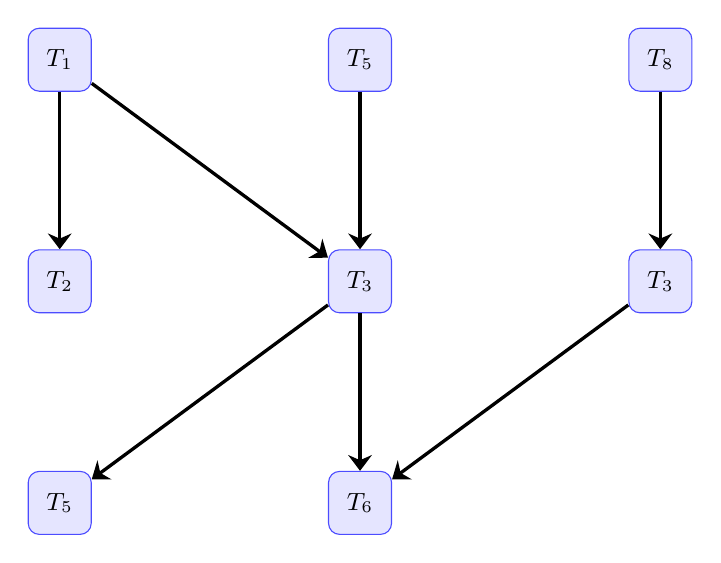
\begin{tikzpicture}[
        >={Stealth[length=2mm, width=3mm]},
        node distance=2cm and 3cm,
        auto
    ]

    % node placement
    \node[task] (T1) {$T_1$};
    \node[task, right=of T1] (T5) {$T_5$};
    \node[task, right=of T5] (T8) {$T_8$};

    \node[task, below=of T1] (T2) {$T_2$};
    \node[task, right=of T2] (T3) {$T_3$};
    \node[task, right=of T3] (T6) {$T_3$};

    \node[task, below=of T2] (T4) {$T_5$};
    \node[task, right=of T4] (T7) {$T_6$};

    % edges
    \draw[->, very thick] (T1) -- (T2);
    \draw[->, very thick] (T1) -- (T3);
    \draw[->, very thick] (T5) -- (T3);
    \draw[->, very thick] (T3) -- (T4);
    \draw[->, very thick] (T3) -- (T7);
    \draw[->, very thick] (T8) -- (T6);
    \draw[->, very thick] (T6) -- (T7);

    \end{tikzpicture}
    \caption{Task graph DAG where $T_i \to T_j$ indicates that task $T_j$ depends on the completion of task $T_i$.}
    \label{fig:task_dag}
\end{figure}

\begin{definition}[\algname{}]
Given an array of tasks and an dictionary of task dependencies, the \algname{} returns an array $L^{*}$ which is the optimal schedule
\end{definition}

This is the definision of the problem

\subsection{Algorithmic Landscape and Background}
\algname{} fits into the landscape of algorithms solving this problem alongside:
\begin{itemize}
    \item \textbf{Naive:} Often provides a baseline, with a running time of $\runtime{\dots}$.
    \item \textbf{\algname{}:} Improved upon Algorithm 1, typically running in $\runtime{\dots}$.
\end{itemize}
Historical work on this problem has focused on \textbf{mention key breakthroughs, e.g., reducing the dependence on a factor like $V$ or $E$ in graphs}.

\textbf{Metrics Comparison:}
\begin{center}
\begin{tabular}{|l|c|c|c|}
\hline
\textbf{Algorithm} & \textbf{Time Complexity} & \textbf{Space Complexity} & \textbf{Notes / Approximation Ratio} \\
\hline
Algorithm 1 & $\runtime{T_1}$ & $\runtime{S_1}$ & Exact/Naive \\
\hline
Algorithm 2 & $\runtime{T_2}$ & $\runtime{S_2}$ & Exact/Standard \\
\hline
\algname{} & $\runtime{T_{alg}}$ & $\runtime{S_{alg}}$ & $\epsilon$-approximation if applicable \\
\hline
\end{tabular}
\end{center}

\section{Algorithm Description and Mechanics}

\subsection{How Does the Algorithm Work?}
\algname{} primarily employs a \textbf{state the algorithmic paradigm, e.g., greedy approach, dynamic programming, divide and conquer}. Its core mechanism revolves around \textbf{a concise explanation of the main idea, e.g., maintaining a set of visited nodes and always exploring the shortest edge to an unvisited node}.

\subsubsection{High-Level Steps}
\begin{enumerate}
    \item Initialization: \dots
    \item Iteration: \dots
    \item Termination: \dots
\end{enumerate}

\subsubsection{Pseudocode}
The formal description of \algname{} is given below.

\begin{algorithm2e}[H]
    \caption{\algname{}}
    \Input{Describe the input structure, e.g., Graph $G=(V, E)$, source node $s$}
    \Output{Describe the output, e.g., Shortest path distance array $D$}            
    \For{$v \in V$}{
        $D[v] \gets \infty$\;
        
        $D[s] \gets 0$\;
        
        $Q \gets \text{PriorityQueue}(V)$\;
        
        \While{$Q$ is not empty}{
            $u \gets \text{ExtractMin}(Q)$\;
            
            \For{each neighbor $v$ of $u$}{
                \If{$D[u] + w(u, v) < D[v]$}{
                    $D[v] \gets D[u] + w(u, v)$\;
                    $\text{DecreaseKey}(Q, v)$\;
                }
            }
        }
    }
\end{algorithm2e}

\subsection{Example Execution}
Consider a small example input: \textbf{Describe the input, e.g., a simple 4-node graph $G$}. 

[Image of Example Graph for Algorithm]


\begin{enumerate}
    \item \textbf{Initial State:} $D = [0, \infty, \infty, \infty]$. Queue $Q=\{s\}$.
    \item \textbf{Step 1:} Extract $s$. Update neighbors \dots
    \item \textbf{Step 2:} Extract \dots
    \item \textbf{Final State:} The resulting array is $D = [\dots]$.
\end{enumerate}

\section{Analysis and Correctness}

\subsection{Why is it Considered Correct?}
The correctness of \algname{} is established through \textbf{state the proof technique, e.g., induction, loop invariants, or exchange arguments}.

\begin{theorem}[Correctness]
\algname{} computes the correct \textbf{solution} for any valid input.
\end{theorem}
\begin{proof}
The proof relies on the \textbf{Loop Invariant}: At the start of each iteration of the main loop, for every node $u$ already extracted from $Q$, $D[u]$ is the true shortest path distance from $s$ to $u$.

\begin{itemize}
    \item \textbf{Initialization:} \dots
    \item \textbf{Maintenance:} \dots
    \item \textbf{Termination:} \dots
\end{itemize}
This completes the proof.
\end{proof}

\subsection{Run-Time Analysis}
The computational complexity of an algorithm is analyzed by counting the number of elementary operations as a function of the input size $N$. For graph algorithms, $N$ is typically $|V|$ (number of vertices) and $|E|$ (number of edges).

\subsubsection{Worst-Case Time Complexity}
The overall complexity is determined by the most time-consuming step:
\begin{itemize}
    \item \textbf{Initialization:} Requires $\runtime{|V|}$ time.
    \item \textbf{Main Loop:} The while loop runs $|V|$ times (once for each vertex).
    \item \textbf{Inner Loop (Relaxation):} The inner loop runs a total of $|E|$ times across all iterations. The cost of operations on the priority queue is key:
    \begin{itemize}
        \item \texttt{ExtractMin}: $\runtime{\log |V|}$ (happens $|V|$ times). Total: $\runtime{|V| \log |V|}$.
        \item \texttt{DecreaseKey}: $\runtime{\log |V|}$ (happens at most $|E|$ times). Total: $\runtime{|E| \log |V|}$.
    \end{itemize}
\end{itemize}

The total worst-case time complexity is dominated by the priority queue operations:
$$T(|V|, |E|) = \runtime{|V| \log |V| + |E| \log |V|} = \runtime{(|V| + |E|) \log |V|}$$

\subsubsection{Practical Run-Times (Optional)}
For practical testing, \algname{} was implemented in \textbf{Language} and run on various datasets.

\textbf{Code Snippet:}
\begin{lstlisting}[caption={Implementation of Key Function}]
def algo_key_function(data):
    # Example logic
    result = 0
    for item in data:
        result += item
    return result
\end{lstlisting}

\textbf{Performance Data:}
\begin{center}
\begin{tabular}{|c|c|c|}
\hline
\textbf{Input Size ($N$)} & \textbf{Theoretical Time (ns)} & \textbf{Observed Time (ms)} \\
\hline
$10^3$ & $T(10^3)$ & $t_1$ \\
\hline
$10^4$ & $T(10^4)$ & $t_2$ \\
\hline
$10^5$ & $T(10^5)$ & $t_3$ \\
\hline
\end{tabular}
\end{center}
The observed data \textbf{confirms/deviates from} the theoretical $\runtime{\dots}$ analysis.

\section{Conclusion}
\algname{} is an efficient solution to the \textbf{Problem Name} problem, achieving a worst-case time complexity of $\runtime{(|V| + |E|) \log |V|}$. Its structure, based on \textbf{paradigm}, ensures its correctness and makes it a foundational algorithm in the study of \textbf{field of study}.

\bibliographystyle{plain}
\bibliography{references} % Create a references.bib file for citations

\end{document}
